\chapter{Subgraphs}
Rishnak found Ajur sleeping with his dog Jura near the cemetery and saw a headstone nearby with the name Schossow. Rishnak recognized the name  from Instant Insanity Puzzle{\footnote{It is also known as Katzenjammer, (Great) Tantalizer, Face-4, Cube-4, Bognar Balls, Taktikolor, Frantic, Diabolical, Damblocks,
Symington's Puzzle. A patent was awarded to  Schossow in 1990}}. Just as Rishnak was thinking it would be an interesting topic to discuss with Ajur, Jura the dog, eager to explore, nudged Ajur. Before long, Ajur and Jura were strolling along a path where Rishnak startled Ajur (as ghosts tend to do). 

Rishnak asked Ajur what he knew about subgraphs. Ajur said that he was familiar with subsets. Since a graph has both a vertex set and edge set, he can deduce what a subgraph is. If a graph $G=(V,E)$ with a vertex set $V$ and an edge set $E$, then take any subset $X$ of $V$ and consider all the edges in E, which has both its end vertices in $X$. Ajur drew this.
\vspace{0.2in}
\\
\noindent
\begin{figure}
\begin{center}
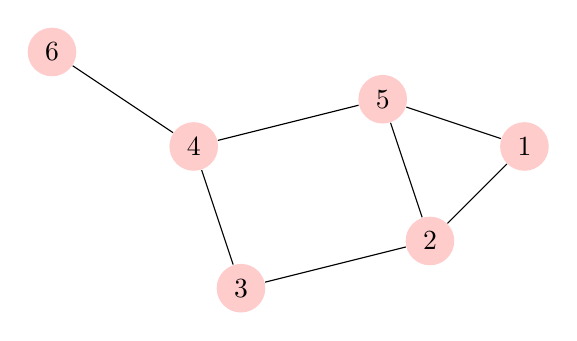
\begin{tikzpicture}
  [scale=.6,auto=left,every node/.style={circle,fill=red!20}]
  \node (n6) at (1,10) {6};
  \node (n4) at (4,8)  {4};
  \node (n5) at (8,9)  {5};
  \node (n1) at (11,8) {1};
  \node (n2) at (9,6)  {2};
  \node (n3) at (5,5)  {3};

  \foreach \from/\to in {n6/n4,n4/n5,n5/n1,n1/n2,n2/n5,n2/n3,n3/n4}
    \draw (\from) -- (\to);

\end{tikzpicture}
\caption{ Example Graph with 6 vertices and 7 edges}\label{3g}
\end{center}
\end{figure}
\\
\noindent
If one took a vertex subset $\{1,2,3,5\}$ of Figure \ref{3g} the subgraph could be as in Figure \ref{3g1}.
\begin{figure}
\begin{center}
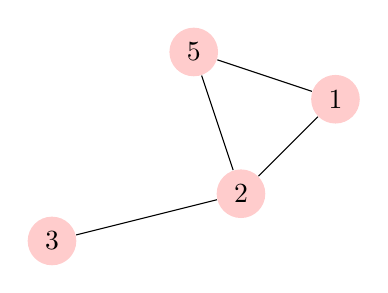
\begin{tikzpicture}
  [scale=.6,auto=left,every node/.style={circle,fill=red!20}]
  %\node (n6) at (1,10) {6};
  %\node (n4) at (4,8)  {4};
  \node (n5) at (8,9)  {5};
  \node (n1) at (11,8) {1};
  \node (n2) at (9,6)  {2};
  \node (n3) at (5,5)  {3};

  \foreach \from/\to in {n5/n1,n1/n2,n2/n5,n2/n3}
    \draw (\from) -- (\to);
\end{tikzpicture}
\caption{Induced Subraph of Figure \ref{3g} Vertices 1,2,3 and 5 are chosen and all the edges between these vertices which are present in the original graph have to be in this subgraph}\label{3g1}
\end{center}
\end{figure}
\\
\noindent
Rishnak laughed and said that the subgraph Ajur drew was called an \textit {induced subgraph} --- that is, all the edges are included in the vertex subset. You have the flexibility of choosing only a subset of these edges. But there is one extra condition: for each edge in the chosen subset of edges, the end vertices should be in the chosen vertex subset. 
\\
\begin{figure}
\begin{center}
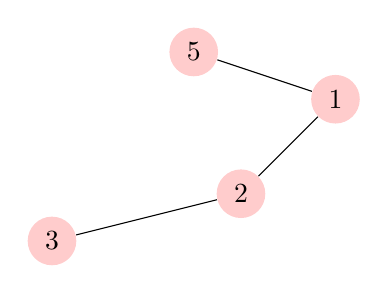
\begin{tikzpicture}
  [scale=.6,auto=left,every node/.style={circle,fill=red!20}]
  %\node (n6) at (1,10) {6};
  %\node (n4) at (4,8)  {4};
  \node (n5) at (8,9)  {5};
  \node (n1) at (11,8) {1};
  \node (n2) at (9,6)  {2};
  \node (n3) at (5,5)  {3};

  \foreach \from/\to in {n5/n1,n1/n2,n2/n3}
    \draw (\from) -- (\to);

\end{tikzpicture}
\caption{A subgraph of Figure \ref{3g}}\label{3g2}
\end{center}
\end{figure}
\\
\noindent
Rishnak illustrated this with the following subgraph example as shown in Figure \ref{3g2}. A subgraph with no vertices and no edges is also an induced subgraph (and subgraph) of any graph.


%Rishnak said that in a graph having $n$ vertices where the vertices are labeled (have a number/name associated with them), then there are at least $2^n$ subgraphs and exactly $2^n$ induced subgraphs.  There are ${n \choose i}$ ways of choosing $i$ vertices from a given set of $n$ vertices. Once the vertices are chosen, the edges are fixed for an induced subgraph. Since $i$ can vary from 0 to $n$, we get $2^n$ induced subgraphs. Since every induced subgraph is a subgraph (and not every subgraph is not an induced subgraph), we have at least $2^n$ subgraphs.  

A walk from a vertex $i$ to a vertex $j$ is an alternating sequence of vertices and edges. Every edge in that walk is incident between vertices preceding and succeeding that edge. For example in Figure \ref{3g},
a walk from vertex 6 to vertex 1 could be 6 (6,4), 4, (4,3), 3, (3,2), 2, (2,1) and 1. The edges are represented as a vertex pair. If those edges are labelled with a name, that label could be used instead. Another walk in Figure \ref{3g} from vertex 6 to vertex 1 could be 6, (6,4), 4, (4,5), 5 (5,1), 1.  The only other condition that the walk has (besides an edge being incident on a preceding and a succeeding vertex) is that all the edges have to be distinct. However the vertices in a walk can be repeated. 
Here is another example Figure \ref{3g3}. A walk from vertex 1 and vertex 8 could be 1, (1,2), 2, (2,4), 4, (4,6), 6, (6,8) and 8. (8,2), 2, (2,3), 3, (3,4), 4, (4,5), 5, (5,6), 6, (6,7), 7, (7,8) and 8. Ajur was naturally getting bored. He interjected that in your walk you have visited all the edges in the graph (shown in Figure \ref{3g3}). Ajur further added that this was similar to the K\"{o}nigsberg Bridge Problem (Figure \ref{kon} mentioned earlier in Chapter 3!).  
\begin{figure}
\begin{center}
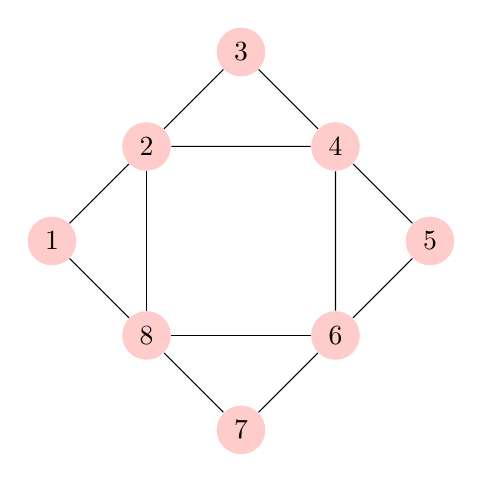
\begin{tikzpicture}
  [scale=.6,auto=left,every node/.style={circle,fill=red!20}]
  \node (n1) at (1,7) {1};
  \node (n2) at (3,9)  {2};
  \node (n3) at (5,11)  {3};
  \node (n4) at (7,9) {4};
  \node (n5) at (9,7)  {5};
  \node (n6) at (7,5)  {6};
  \node (n7) at (5,3)  {7};
  \node (n8) at (3,5)  {8};

  \foreach \from/\to in {n1/n2,n1/n8,n2/n3,n2/n4,n2/n8,n3/n4,n4/n5,n4/n6,n5/n6,n6/n7,n6/n8,n7/n8}
    \draw (\from) -- (\to);

\end{tikzpicture}
\caption{ Example Graph with 8 vertices and 12 edges}\label{3g3}
\end{center}
\end{figure}
\\

If the starting and ending vertices in a walk are the same, it is known as a closed walk. If all the edges in a closed walk are distinct, then it is known as a cycle. 
Ajur had heard of this from his friends.
Rishnak asked Ajur to list two cycles from Figure \ref{3g3}. Ajur had no trouble at all, in listing two cycles as (1,(1,2),2,(2,8),8,(8,1),1) and (2,(2,4),4,(4,6),6,(6,8),8,(8,2)2). Often the edges are omitted, and the cycles are written as (1,2,8,1) and (2,4,6,8,2).  Of course, a cycle and a walk are examples of subgraphs with some added conditions. These added conditions make the study of subgraphs very interesting. If in a cycle, all the vertices of the original graph are present, then that cycle is known as a Hamiltonian Cycle. For example in Figure \ref{3g3} the cycle (1,2,3,4,5,6,7,8,1) is a Hamiltonian Cycle of Figure \ref{3g4}. If all the edges in a walk are distinct then it is known as a path. Ajur gave the following examples for a path in Figure \ref{3g3} as (1,(1,2),2,(2,3),3) or simply as (1,2,3), Figure \ref{3g5}. If there is a path between every pair of vertices in a subgraph, then the subgraph is said to be connected. If a subgraph contains no cycles and is connected, the subgraph is a tree. If such a tree contains all vertices then it is known as spanning tree, Figure \ref{3g6}.  A subgraph in which the degree of every vertex is 1 is called a matching. An example of a subgraph (which is a matching for Figure \ref{3g3}) is in Figure \ref{3g7}. If the subgraph contains all vertices and the degree of every vertex is one, then it is called as Perfect matching. An example of a subgraph that is a perfect matching for Figure~\ref{3g3} is in Figure \ref{3g8}. Rishnak asked Ajur how many perfect matchings there are in Figure \ref{3g3}. Ajur thought a bit. He saw vertices 1, 3, 5 and 7 hae degree 2. Hence one of those incident on 1, 3, 5 and 7 have to be selected. Hence he replied that there are exactly two perfect matchings in Figure \ref{3g3}. 
\\
\begin{figure}
\begin{center}
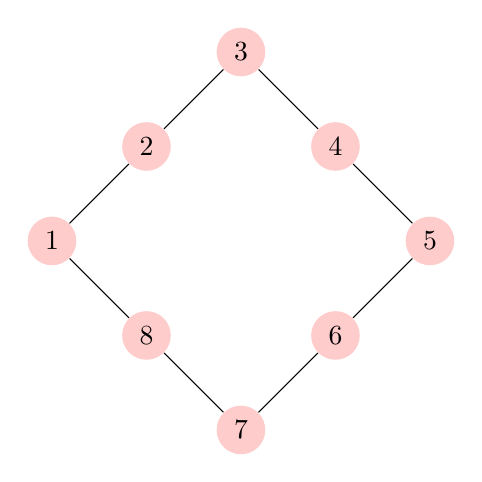
\begin{tikzpicture}
  [scale=.6,auto=left,every node/.style={circle,fill=red!20}]
  \node (n1) at (1,7) {1};
  \node (n2) at (3,9)  {2};
  \node (n3) at (5,11)  {3};
  \node (n4) at (7,9) {4};
  \node (n5) at (9,7)  {5};
  \node (n6) at (7,5)  {6};
  \node (n7) at (5,3)  {7};
  \node (n8) at (3,5)  {8};

  \foreach \from/\to in {n1/n2,n1/n8,n2/n3,n3/n4,n4/n5,n5/n6,n6/n7,n7/n8}
    \draw (\from) -- (\to);

\end{tikzpicture}
\caption{ A subgraph which is a Hamiltonian Cycle}\label{3g4}
\end{center}
\end{figure}

\begin{figure}
\begin{center}
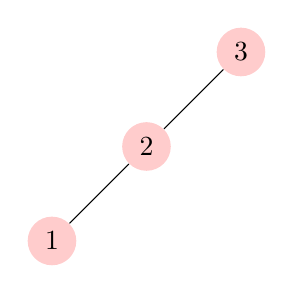
\begin{tikzpicture}
  [scale=.6,auto=left,every node/.style={circle,fill=red!20}]
  \node (n1) at (1,7) {1};
  \node (n2) at (3,9)  {2};
  \node (n3) at (5,11)  {3};


  \foreach \from/\to in {n1/n2,n2/n3}
    \draw (\from) -- (\to);

\end{tikzpicture}
\caption{ A subgraph which is a tree}\label{3g5}
\end{center}
\end{figure}

\begin{figure}
\begin{center}
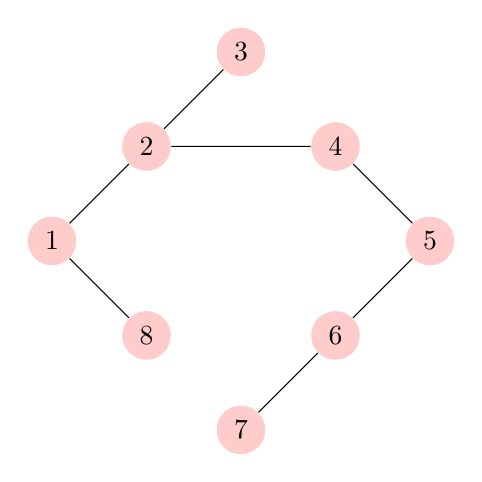
\begin{tikzpicture}
  [scale=.6,auto=left,every node/.style={circle,fill=red!20}]
  \node (n1) at (1,7) {1};
  \node (n2) at (3,9)  {2};
  \node (n3) at (5,11)  {3};
  \node (n4) at (7,9) {4};
  \node (n5) at (9,7)  {5};
  \node (n6) at (7,5)  {6};
  \node (n7) at (5,3)  {7};
  \node (n8) at (3,5)  {8};

  \foreach \from/\to in {n1/n2,n1/n8,n2/n3,n2/n4,n4/n5,n5/n6,n6/n7}
    \draw (\from) -- (\to);

\end{tikzpicture}
\caption{ A subgraph which is a spanning tree}\label{3g6}
\end{center}
\end{figure}

\begin{figure}
\begin{center}
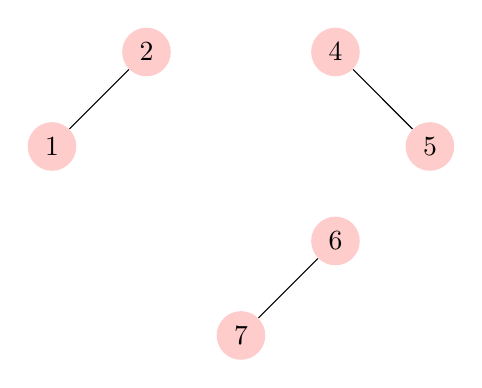
\begin{tikzpicture}
  [scale=.6,auto=left,every node/.style={circle,fill=red!20}]
  \node (n1) at (1,7) {1};
  \node (n2) at (3,9)  {2};
  %\node (n3) at (5,11)  {3};
  \node (n4) at (7,9) {4};
  \node (n5) at (9,7)  {5};
  \node (n6) at (7,5)  {6};
  \node (n7) at (5,3)  {7};
  %\node (n8) at (3,5)  {8};

  \foreach \from/\to in {n1/n2,n4/n5,n6/n7}
    \draw (\from) -- (\to);

\end{tikzpicture}
\caption{ A subgraph which is a matching}\label{3g7}
\end{center}
\end{figure}

\begin{figure}
\begin{center}
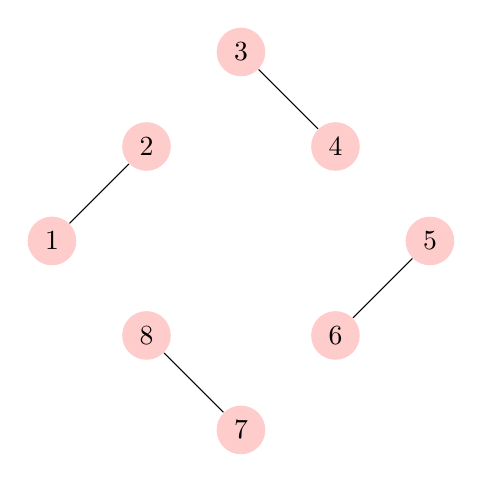
\begin{tikzpicture}
  [scale=.6,auto=left,every node/.style={circle,fill=red!20}]
  \node (n1) at (1,7) {1};
  \node (n2) at (3,9)  {2};
  \node (n3) at (5,11)  {3};
  \node (n4) at (7,9) {4};
  \node (n5) at (9,7)  {5};
  \node (n6) at (7,5)  {6};
  \node (n7) at (5,3)  {7};
  \node (n8) at (3,5)  {8};

  \foreach \from/\to in {n1/n2,n3/n4,n5/n6,n7/n8}
    \draw (\from) -- (\to);

\end{tikzpicture}
\caption{ A subgraph which is a perfect matching}\label{3g8}
\end{center}
\end{figure}

\vspace{3in}
A graph is connected if there is a path between every pair of vertices in that graph. Otherwise the graph is disconnected,  Here is an example of a connected graph, Figure \ref{3g9}. Here is an example of a graph that is not connected, Figure \ref{3g10}
\begin{figure}
\begin{center}
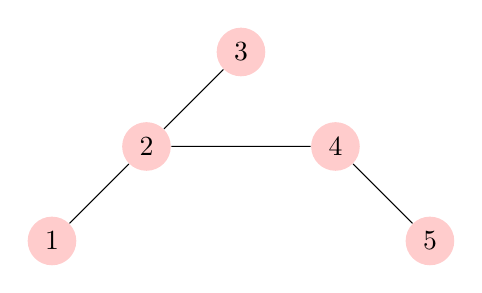
\begin{tikzpicture}
  [scale=.6,auto=left,every node/.style={circle,fill=red!20}]
  \node (n1) at (1,7) {1};
  \node (n2) at (3,9)  {2};
  \node (n3) at (5,11)  {3};
  \node (n4) at (7,9) {4};
  \node (n5) at (9,7)  {5};
\foreach \from/\to in {n1/n2,n2/n3,n2/n4,n4/n5}
    \draw (\from) -- (\to);

\end{tikzpicture}
\caption{ A connected graph}\label{3g9}
\end{center}
\end{figure}

\begin{figure}
\begin{center}
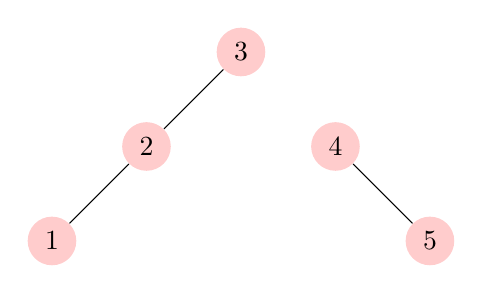
\begin{tikzpicture}
  [scale=.6,auto=left,every node/.style={circle,fill=red!20}]
  \node (n1) at (1,7) {1};
  \node (n2) at (3,9)  {2};
  \node (n3) at (5,11)  {3};
  \node (n4) at (7,9) {4};
  \node (n5) at (9,7)  {5};
\foreach \from/\to in {n1/n2,n2/n3,n4/n5}
    \draw (\from) -- (\to);

\end{tikzpicture}
\caption{ A graph that is not connected}\label{3g10}
\end{center}
\end{figure}
\vspace{3in}

\textbf{Question for the third day:} Rishnak asked Ajur to list the cycles in the following graph Figure \ref{day3g1} 

\begin{figure}
\begin{center}
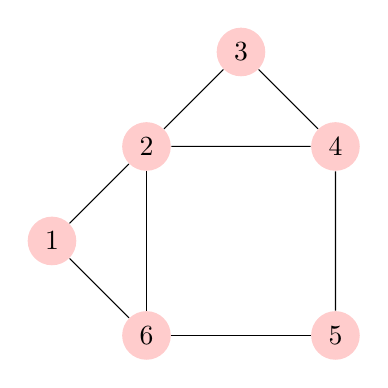
\begin{tikzpicture}
  [scale=.6,auto=left,every node/.style={circle,fill=red!20}]
  \node (n1) at (1,7) {1};
  \node (n2) at (3,9)  {2};
  \node (n3) at (5,11)  {3};
  \node (n4) at (7,9) {4};
  \node (n5) at (7,5)  {5};
  \node (n6) at (3,5)  {6};

  \foreach \from/\to in {n1/n2,n1/n6,n2/n3,n2/n4,n2/n6,n3/n4,n4/n5,n5/n6}
    \draw (\from) -- (\to);

\end{tikzpicture}
\caption{ How many Cycles are there in this Graph?}\label{day3g1}
\end{center}
\end{figure}

\textbf{Answer:} Ajur listed the 6 cycles as follows:
\begin{enumerate}
    \item Cycle of length 3 (two namely  (1,2,6), (2,3,4)
    \item Cycle of length 4 (one namely) (2,4,5,6)
    \item Cycle of length 5 (two namely) (2,3,4,,5,6), (1,2,4,5,)
    \item Cycle of length 6 (one namely) (1,2,3,4,5,6)
\end{enumerate}
Rishank  was pleased and noticed that Ajur was getting restless, and so was Jura, and so they called it a day.